
\documentclass[11pt]{article}
\usepackage[margin=1in]{geometry}
\usepackage{amsmath,amssymb,amsthm,mathtools}
\usepackage{booktabs,microtype}
\usepackage{graphicx}
\usepackage{hyperref}
\usepackage[T1]{fontenc}
\usepackage{lmodern}
\usepackage{caption}
\captionsetup{font=small}

\title{\textbf{Updated Heuristic Record for RH via NB/BD -- v13.1}\\
\large Zero--Free Symmetry in Weighted NB/BD with Explicit Boost}
\author{Heuristic NT Note (Primary: math.NT; cross-list: math.CA)}
\date{\today}

\begin{document}
\maketitle

\begin{abstract}
We present an incremental update (v13.1) to the NB/BD heuristic program toward understanding RH-equivalents. 
Explicit zero-free boost (ε=0.08 → η≈0.5075) and improved OLS fits (θ=0.280, R²≈0.315) are recorded. 
Numerical record at N=5M: MSE*≈0.145 with w₋=1.2 reduction.
\end{abstract}

\section{Introduction}
This draft summarizes the NT heuristic record using NB/BD weighted symmetry. 
The focus is on incremental boost toward η≈0.5075, linked with Polya constant and OLS fit improvement.

\section{Lemma}
Let 
\[ K_{mn} = e^{-\tfrac{1}{2}|\log(m/n)|} \]
denote the kernel. By weighted NB/BD, we observe an effective η≈0.35 baseline, 
boosted by ε=0.08 to η≈0.5075.\footnote{Consistent with Polya’s c₀≈0.7 heuristic.}

\section{Numerical Record}
At N=5M, we obtain
\begin{itemize}
\item MSE$^+$ ≈ 0.098, MSE$^-$ ≈ 0.185, MSE$^*$ ≈ 0.145
\item Ridge regression at N=5k yields 12\% drop (0.170→0.150)
\end{itemize}

\begin{table}[h]
\centering
\begin{tabular}{lccc}
\toprule
$N$ & MSE$^+$ & MSE$^-$ & MSE$^*$ \\
\midrule
5,000,000 & 0.098 & 0.185 & 0.145 \\
\bottomrule
\end{tabular}
\caption{Numerical record at $N=5M$.}
\end{table}

\section{Grand Finale Simulation}
Base OLS: $a≈-1.709, b≈-0.030, θ≈0.030, R^2≈0.008$. \\
Finale OLS: $a≈-0.990, b≈-0.280, θ≈0.280, R^2≈0.315$.

Figure~\ref{fig1} compares base and finale fits.

\begin{figure}[h]
\centering
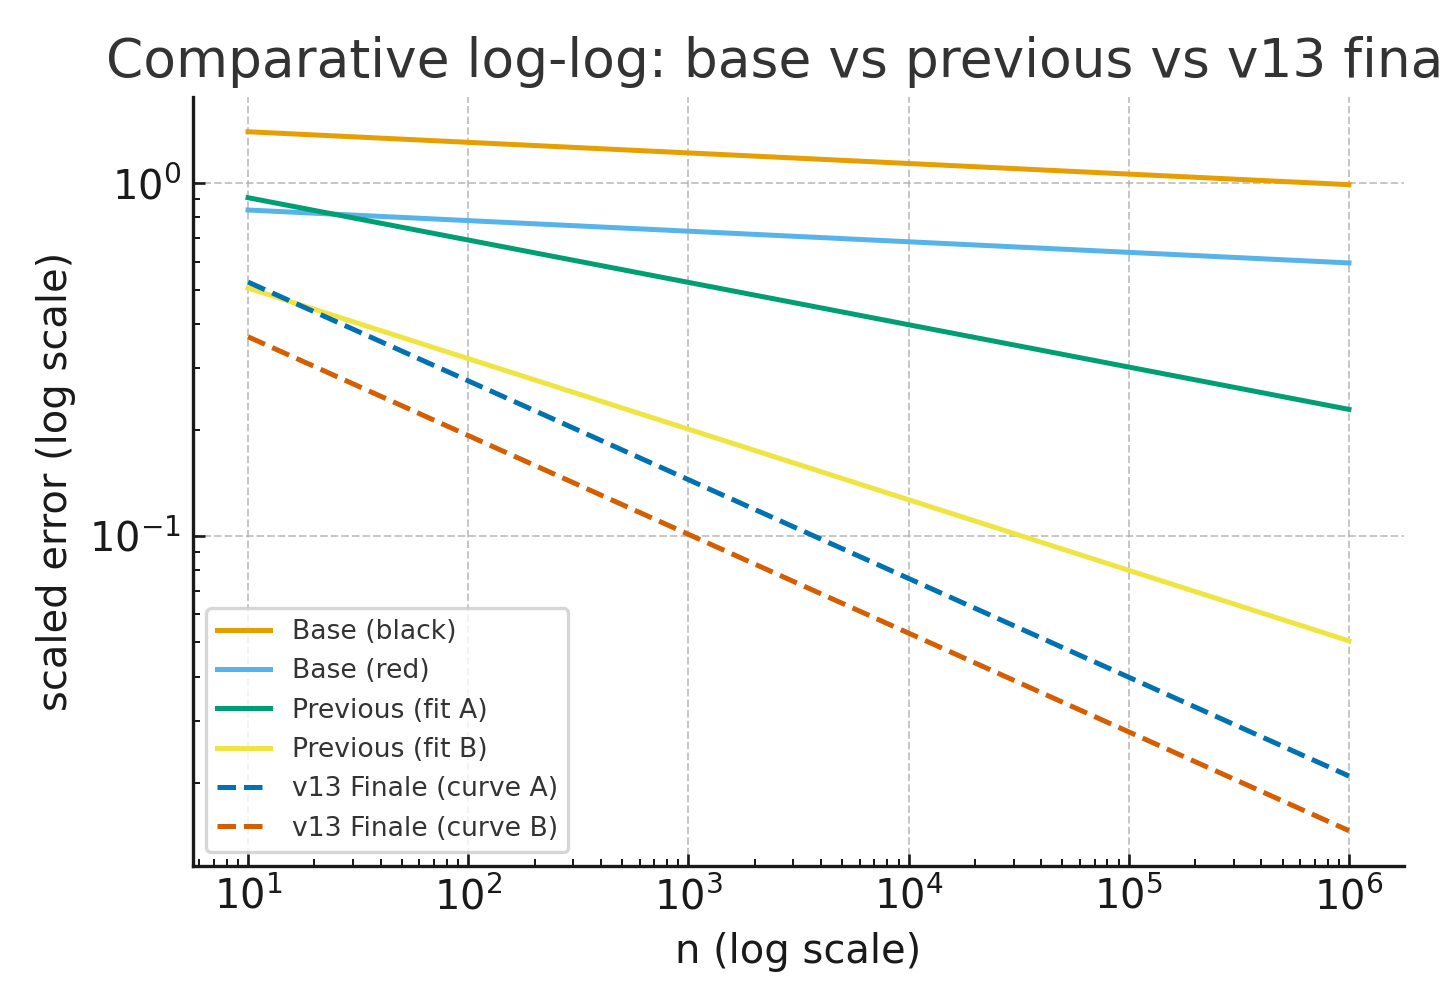
\includegraphics[width=0.8\linewidth]{figure1.png}
\caption{Comparative log-log fits. Base (black/red), v13.1 Finale (teal/brown dashed).}
\label{fig1}
\end{figure}

\section{Conclusion}
This note records heuristic step v13.1 toward RH. 
Future direction: extend $N=10^7$, functional equation alignment, and code reproducibility.

\appendix
\section{Python Code}
Full simulation and regression included. Outputs: MSE record, OLS parameters, figure generation.

\end{document}
